\documentclass{article}

\usepackage{geometry}
\usepackage{tikz}
\usepackage{rubikcube,rubikrotation,rubikpatterns}
\usepackage{graphicx}
\usepackage{fancyhdr}
\usepackage{polyglossia}
\usepackage{geometry}
\usepackage{lastpage}
\usepackage{fontspec}
\usepackage{subfigure}
\usepackage{subcaption}
\usepackage{listings}
\usepackage{xcolor}
\usepackage{hyperref}
\setlength{\parindent}{0cm}

\geometry{a4paper,hmargin=0.75in,vmargin={1.1in,0.6in},head=75pt,foot=45pt, left=2.5cm, right=2.5cm, includefoot, footskip=60pt}

\pagestyle{fancy}

\fancyhead[L]{\leftmark}
\fancyhead[C]{}
\fancyhead[R]{\textit{Tutorial 3BLD}}

\fancyfoot[C]{}
\fancyfoot[R]{Pàg \thepage\ / \pageref{LastPage}}

\setlength{\headsep}{1cm}

\renewcommand{\headrulewidth}{1pt}
\renewcommand{\footrulewidth}{0.4pt}

\renewcommand{\baselinestretch}{1.5}

% Estil dels links

\hypersetup{
    colorlinks=true,
    linkcolor=black,
    urlcolor=cyan,
    urlbordercolor={0 1 0}
}

\fontsize{12}{14} 
\setmainfont{arial}

\setdefaultlanguage{catalan}


\title{\textbf{TUTORIAL DE 3BLD}}
\author{Pol Sances Guirao}
\date{2023}

\begin{document}

\thispagestyle{empty}
\maketitle
\newpage

\thispagestyle{empty}
\tableofcontents
\newpage

\thispagestyle{empty}
Aquest tutorial està pensat per a persones que ja tenen un domini mínim del cub, es recomana que les persones sapiguen fer el cub de Rubik ja que facilita molt el procés.


\newpage
\section{Coses a saber abans de començar}

\subsection{Notació dels Moviments}

El cub de rubik es resol gràcies a identificar patrons i executar algoritmes que resolen aquests patrons, aquests algoritmes han d'estar escrits en alguna part per poder-los memoritzar i per això estaà la notació del cub de rubik.
\\\\La notació consta de 6 moviments (F,B,R,L,U,D), que correspon a (Front, Back, Right, Left, Up, Down) que son les respectives direccions en anglés. Per exemple si faig el moviment F gira la cara front la que està més propera a la nostra visió, en sentit horari, en canvi si fós F' seria antihorari. En les figures següents es mostra una respresentació gràfica per a cada capa.
\\\\És un concepte difícil d'entendre però de manera simplificada és girar la cara en sentit horari i antihorari desde la cara que vulguis. En les figures següents es mostra una respresentació gràfica per a cada capa.

\begin{figure}[htbp]
    \centering
    \begin{subfigure}
        \centering\RubikCubeSolvedWY
        \RubikRotation{Y,F}
        \ShowCube{7cm}{0.5}{\DrawRubikCubeLU}
    \end{subfigure}
    \begin{subfigure}
        \centering\RubikCubeSolvedWY
        \RubikRotation{Y,Fp}
        \ShowCube{7cm}{0.5}{\DrawRubikCubeLU}
    \end{subfigure}
    \caption{Exemples de Movimients F y F'}
\end{figure}

\begin{figure}[htbp]
    \centering
    \begin{subfigure}
        \centering\RubikCubeSolvedWY
        \RubikRotation{Y,B}
        \ShowCube{7cm}{0.5}{\DrawRubikCubeLU}
    \end{subfigure}
    \begin{subfigure}
        \centering\RubikCubeSolvedWY
        \RubikRotation{Y,Bp}
        \ShowCube{7cm}{0.5}{\DrawRubikCubeLU}
    \end{subfigure}
    \caption{Exemples de Movimients B y B'}
\end{figure}

\begin{figure}[htbp]
    \centering
    \begin{subfigure}
        \centering\RubikCubeSolvedWY
        \RubikRotation{Y,R}
        \ShowCube{7cm}{0.5}{\DrawRubikCubeLU}
    \end{subfigure}
    \begin{subfigure}
        \centering\RubikCubeSolvedWY
        \RubikRotation{Y,Rp}
        \ShowCube{7cm}{0.5}{\DrawRubikCubeLU}
    \end{subfigure}
    \caption{Exemples de Movimients R y R'}
\end{figure}

\begin{figure}[htbp]
    \centering
    \begin{subfigure}
        \centering\RubikCubeSolvedWY
        \RubikRotation{Y,L}
        \ShowCube{7cm}{0.5}{\DrawRubikCubeLU}
    \end{subfigure}
    \begin{subfigure}
        \centering\RubikCubeSolvedWY
        \RubikRotation{Y,Lp}
        \ShowCube{7cm}{0.5}{\DrawRubikCubeLU}
    \end{subfigure}
    \caption{Exemples de Movimients L y L'}
\end{figure}

\begin{figure}[htbp]
    \centering
    \begin{subfigure}
        \centering\RubikCubeSolvedWY
        \RubikRotation{Y,U}
        \ShowCube{7cm}{0.5}{\DrawRubikCubeLU}
    \end{subfigure}
    \begin{subfigure}
        \centering\RubikCubeSolvedWY
        \RubikRotation{Y,Up}
        \ShowCube{7cm}{0.5}{\DrawRubikCubeLU}
    \end{subfigure}
    \caption{Exemples de Movimients U y U'}
\end{figure}

\begin{figure}[ht!]
    \centering
    \begin{subfigure}
        \centering\RubikCubeSolvedWY
        \RubikRotation{Y,D}
        \ShowCube{7cm}{0.5}{\DrawRubikCubeLU}
    \end{subfigure}
    \begin{subfigure}
        \centering\RubikCubeSolvedWY
        \RubikRotation{Y,Dp}
        \ShowCube{7cm}{0.5}{\DrawRubikCubeLU}
    \end{subfigure}
    \caption{Exemples de Movimients D y D'}
    \label{fig:d-d'}
\end{figure}

\subsection{Interpretar el concepte del cub}

La manera correcta d'interpretar el cub és pensar en el funcionament, com si el desmuntessis, ja que consta de 12 arestes i 8 cantonades, a més a més dels 6 centres que no poden permutar\footnote{Intercanvi de posició amb una altre peça i de l'ordre de tot el conjunt} amb cap altra peça ja que només roten.

\begin{figure}[h!]
    \centering
    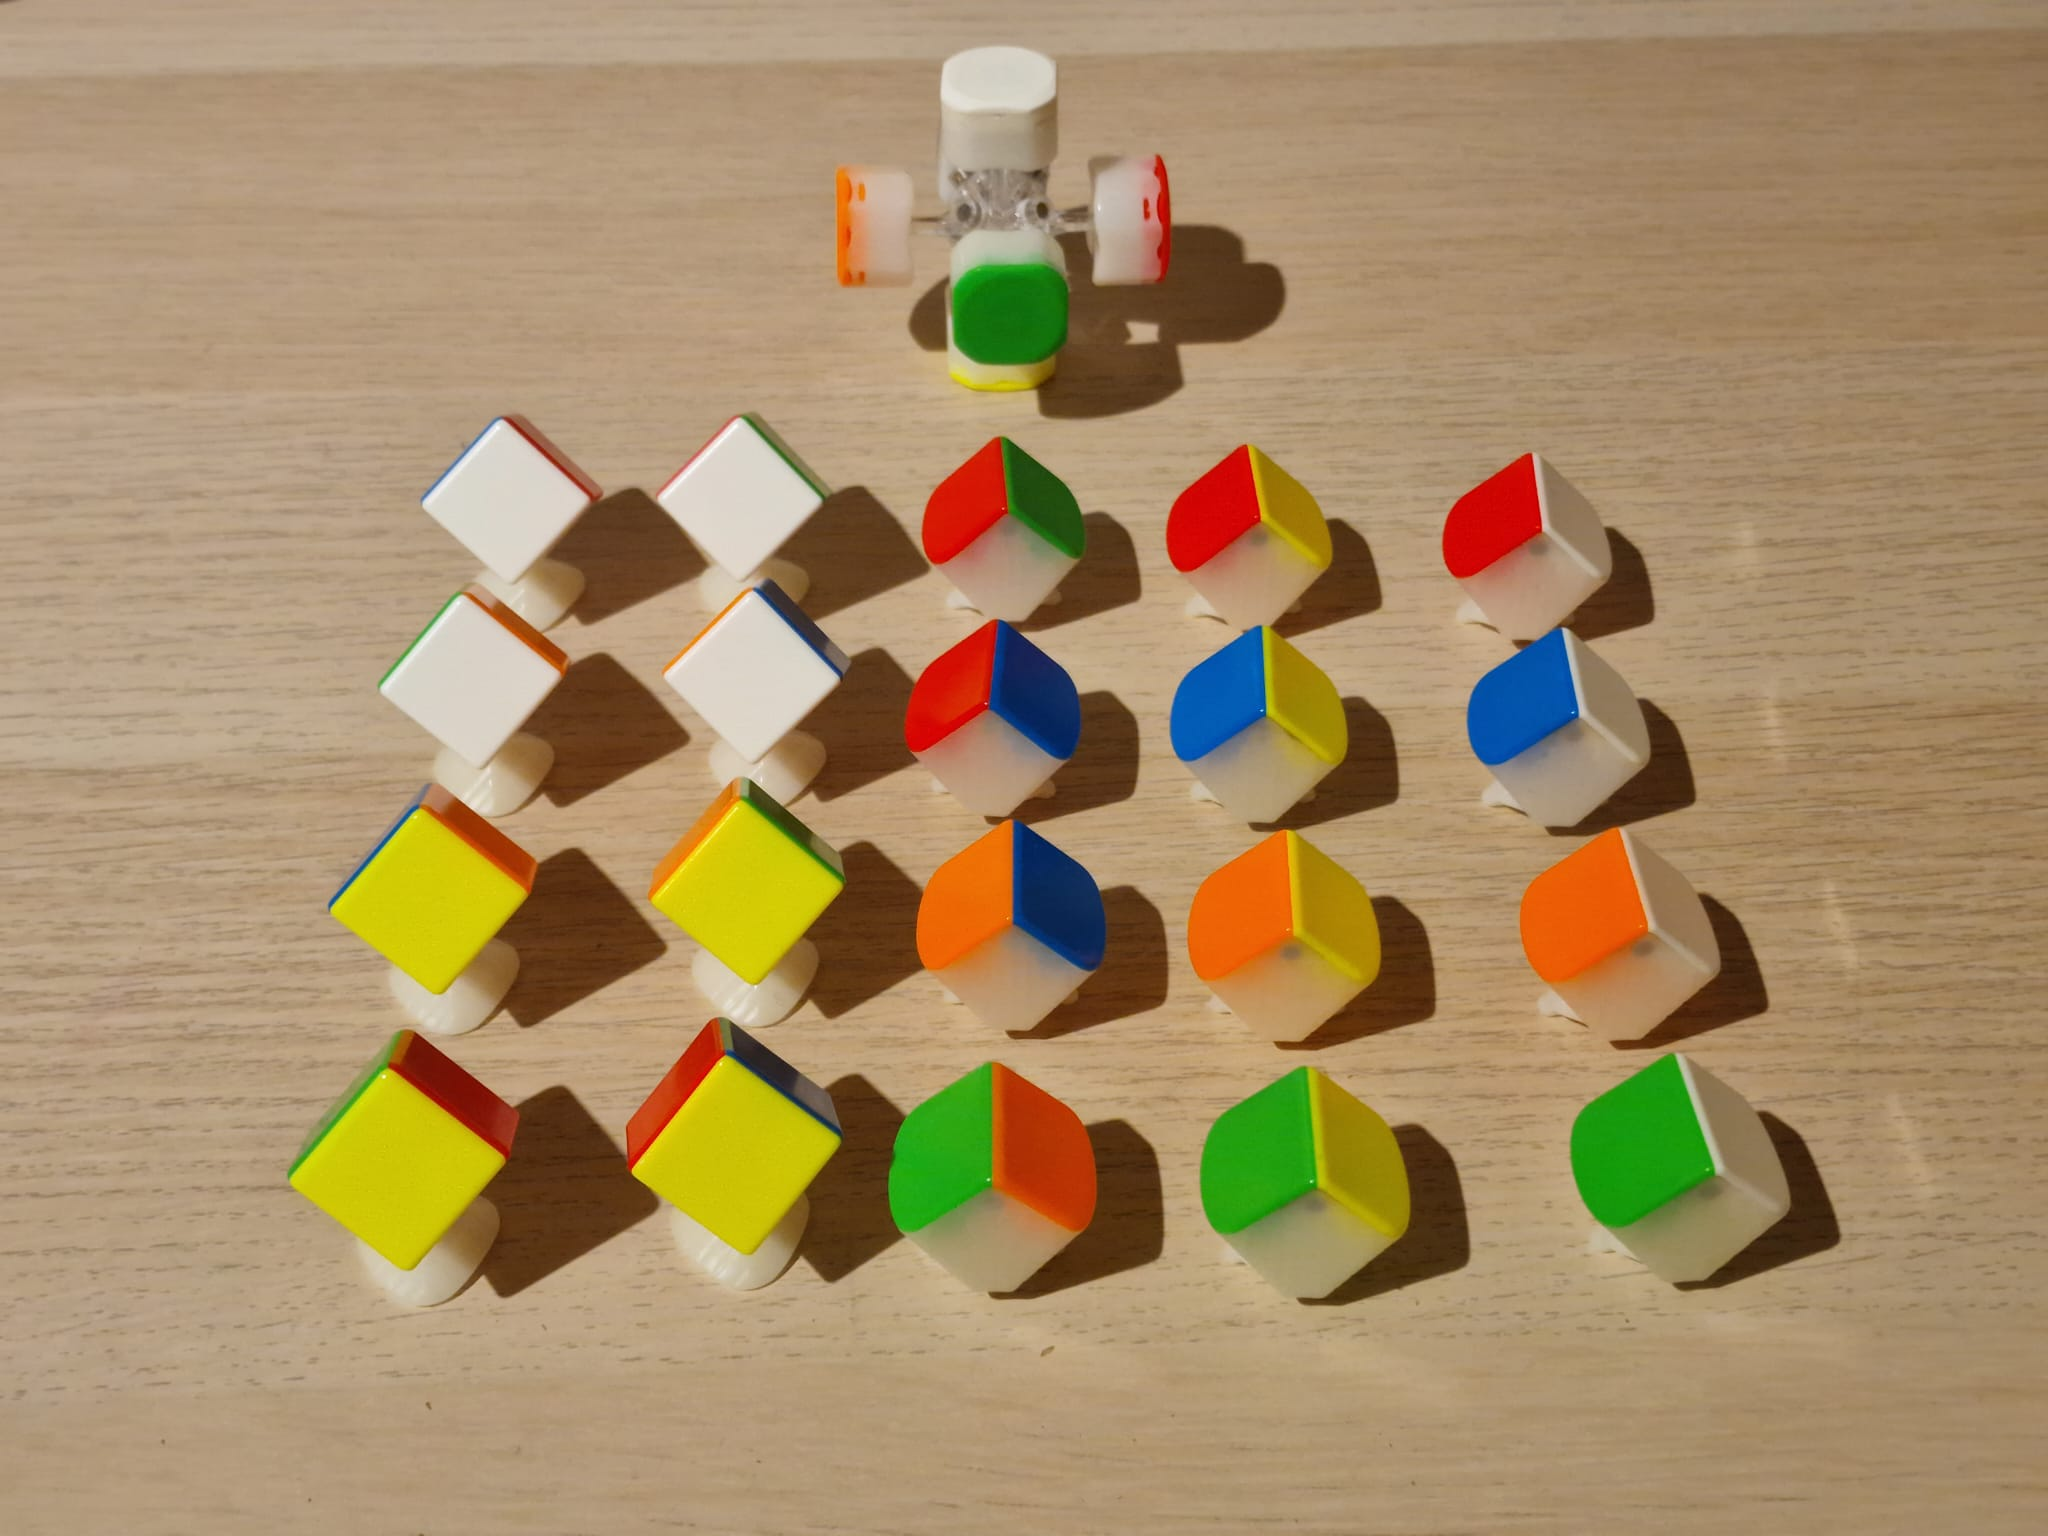
\includegraphics[width=7cm]{img/figures/cub-desmontat.jpg}
    \caption{Cub Desmuntat}
    \label{fig:cub-desmuntat}
\end{figure}


\newpage
\section{El Concepte de 3BLD}

Per començar cal entendre el funcionament d'una resolució de blind, primer el cub és barrejat per una persona i el posa dins d'una capsa o un cube cover\footnote{Un cube cover és una tapa per cubs feta de cartró i que s'utlitza a les competicions}, després es col·loca a la taula boca avall i la persona que l'ha de resoldre es pren el seu temps per respirar. 
Un cop fet això la persona que resol el cub encén el timer i destapa el cub, de manera que el temps comença a comptar i es comença a memoritzar. Un cop acabada la memorització el que resol el cub es tapa els ulls amb un antifaç i comença a resoldre el cub, mentre que una persona externa li posa una cartiluna entre el cub i la seva cara per evitar trampes i mirar per sota de l'antifaç.
Tots aquests passos s'han d'executar perfectament per asegurar-se de la resolució compti.

\begin{figure}[ht]
    \centering
    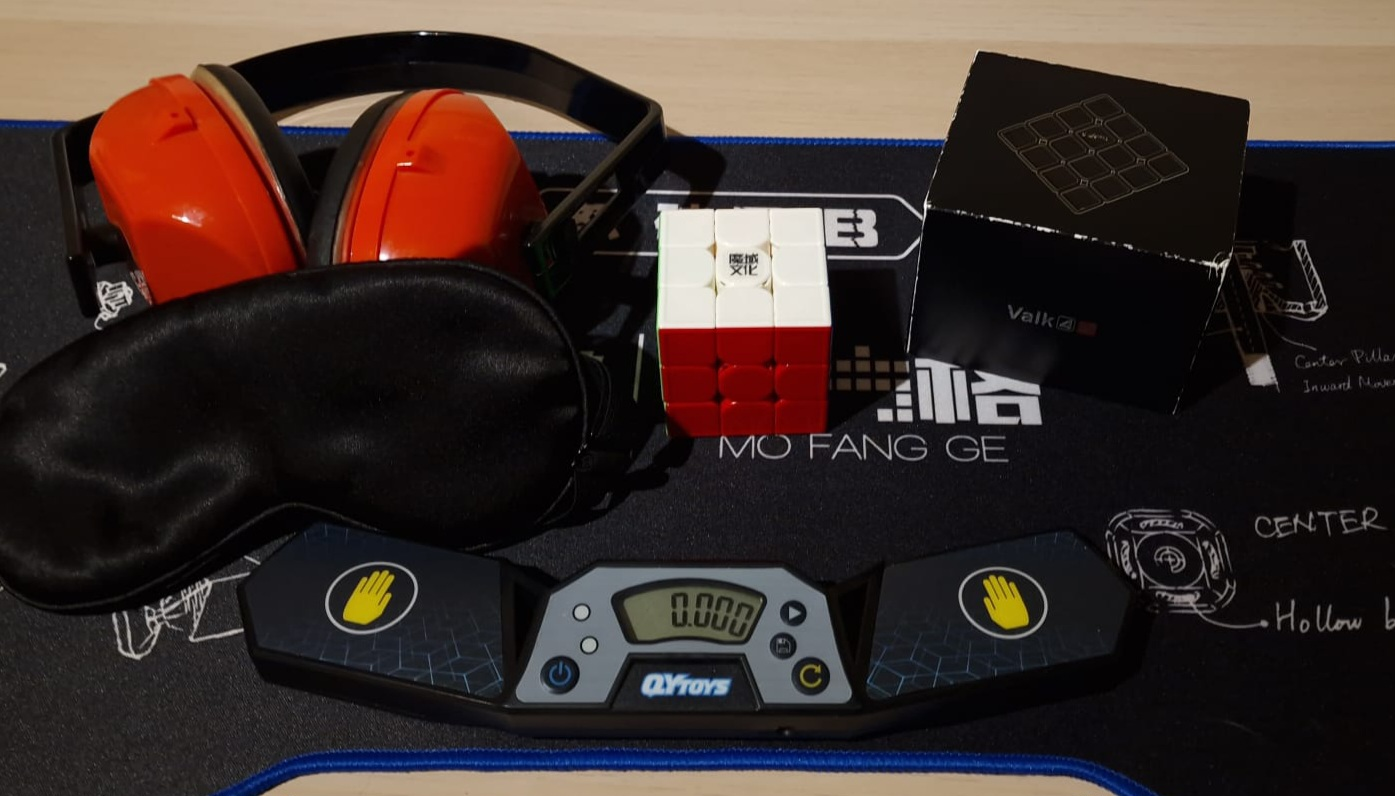
\includegraphics[width=12cm]{img/figures/materials-bld.jpg}
\caption{Materials necessaris per poder executar blind}
    \label{fig:materials-bld}
\end{figure}


\vspace{0.5cm}
\subsection{Fases de la Resolució}

Com ja he esmentat a la seccio anterior, completar el cub de Rubik amb els ulls tancats, es divideix en dos grans fases, memorització i execució. I dins d'aquestes fases hi han diferents procediments per poder aconseguir fer-ho correctament.

\subsection{Memorització}


En aquesta fase com ja ho diu el seu nom has de memoritzar el cub. La manera de memoritzar no és la més convencional ja que no memoritzes color sinó peces i com que hem d'interpretar el cub  com si fossin 20 peces el que fem es donar-li una lletra per la qual pots identificar a cada peça. Fent aquestes conversions has d'arribar a tenir el teu propi esquema de lletres, el que utilitzo jo és el de la figura \ref{fig:letter-scheme}, i el pots agafar com a plantilla per fer el teu o directament utilitzar-lo ja que si t'acostumes no et limitarà res durant el procés.

\begin{figure}[ht]
    \centering
    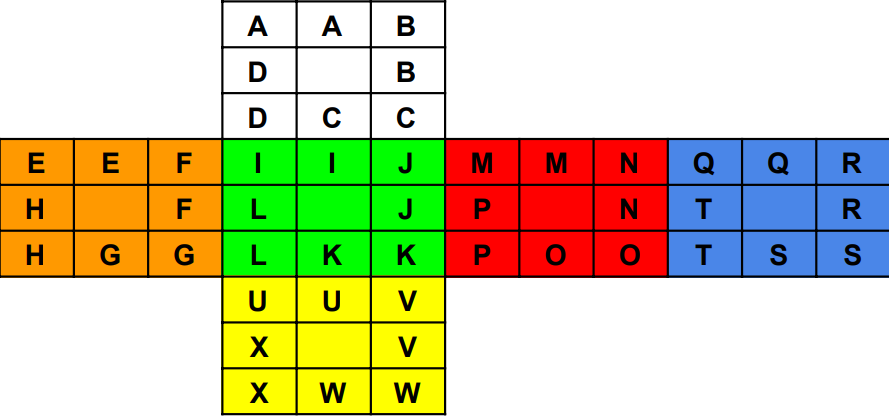
\includegraphics[width=12cm]{img/figures/letter-scheme.png}
\caption{Esquema de Lletres}
    \label{fig:letter-scheme}
\end{figure}

Hi han lletres repetides perquè primer memoritzes arestes i després cantonades, aquestes lletres a l'hora de memoritzar-les, no les memoritzes a força bruta, sinó que les converteixes en paraules que puguis convertir en imatges per poder entrecordar-te. Sembla molt complex però no ho és com es pot veure en el següent exemple.
Per practicar aquesta transformació d'imatges pots anar a la pàgina web \href{https://polsances13.github.io/roadto3bld/App.Html}{roadto3bld} on podràs veure el codi de la app i on hi haurà un link a github on podràs descarregar i utilitzar l'app.
\vspace{0.25cm}

$$ \textrm{Haig de memoritzar les lletres R i B    }  \rightarrow \textrm{   RedBull} $$
$$ \textrm{Haig de memoritzar les lletres A i C   }  \rightarrow \textrm{   Aire Acondicionat (AC és el símbol)} $$

Llavors has de tenir per a cada parell de lletres una paraula clau per memoritzarles ràpidament. Et pots inspirar en les d'algú, com les meves de les taules \ref{tla:lletres-1} al final del document, però aquestes si que no les hauries de copiar, ja que aquestes paraules han de ser les que primer et vinguin al cap pensant en les dues lletres, és un treball una mica pesat però amb el temps dona el seu fruit.
No hi ha secret per integrar aquestes paraules a la teva ment, el que has de fer és practicar, practicar i practicar, i amb el temps et sortirà sol.

\subsection{Execució}

A diferència de una resolució normal, a l'hora d'executar els moviments tu no pots rotar el cub, perquè tens que actuar segons les lletres que has memoritzat i si rotes el cub canvies la posició de les peces respecte a les lletres indirectament. 
Per tant només fas moviments de les capes. Els algoritmes per intercanviar les peces només interfereixen en les lletres que has memoritzat i deixent la resta del cub exactament igual quan fas els passos. Per començar a fer el cub has d'aprendre el mètode principants que explicaré a la següent secció.
Durant l'execució se segueix l'ordre CEEC que diu que memoritzes cantonades, després arestes, executes arestes i després executes cantonades.


\newpage
\section{El mètode principiants "Old Pochmann"}

El métode principiants o Old Pochmann és un mètode pel qual intercanvies les peces que vols una a una, és a dir, que mires la peça que primer has memoritzat i la canvies per la peça que està al seu lloc i així ja tens una peça que està al seu lloc i una altra que has de col·locar, i així succesivament.
Aquesta peça sobre la que sempre estàs treballant es diu "Buffer".El mètode és el mateix concepte tant per arestes com cantonades però el dividirem en dos perquè l'explicació sigui més fàcil.

\subsection{Arestes}

En les arestes el buffer serà la peça BM, (l'aresta blanca-vermella), i a l'hora de memoritzar començarem des d'allà. Un cop memoritzat un "setup move", que consisteix en un moviment que posa la peça que vols intercanviar en el lloc AD, (l'aresta blanca-taronja) i seguit del setup move farem l'algoritme d'intercanvi del mètode, després desfarem el setup movem executant-lo però a revés.


$$ \textrm{Algortime d'intercanvi} \rightarrow \textrm{R U R' U' R' F R2 U' R' U' R U R' F'} $$

Els setups moves més òptims per cada peça de les arestes són els següents:

\begin{table}[h]
    \begin{minipage}{.5\linewidth}
        \centering
        \begin{tabular}{|c|c|}
            \hline
            A & Lw2 D' L2     \\ 
            \hline
            B & buffer        \\ 
            \hline
            C & Lw2 D L2      \\
            \hline
            D & Fer algoritme \\ 
            \hline
            E & L Dw' L       \\ 
            \hline
            F & Dw' L         \\ 
            \hline
            G & L' Dw' L      \\ 
            \hline
            H & Dw L'         \\ 
            \hline
            I & Lw D' L2      \\ 
            \hline
            J & Dw2 L         \\ 
            \hline
            K & Lw D L2       \\ 
            \hline
            L & L'            \\ 
            \hline
        \end{tabular}
    \end{minipage}
    \begin{minipage}{.5\linewidth}
        \centering
        \begin{tabular}{|c|c|}
            \hline
            M & buffer        \\ 
            \hline
            N & Dw L          \\ 
            \hline
            O & D2 L' Dw' L   \\ 
            \hline
            P & Dw' L'        \\ 
            \hline
            Q & Lw' D L2      \\ 
            \hline
            R & L             \\ 
            \hline
            S & Lw' D' L2     \\ 
            \hline
            T & Dw2 L'        \\ 
            \hline
            U & D' L2         \\ 
            \hline
            V & D2 L2         \\ 
            \hline
            W & D L2          \\ 
            \hline
            X & L2            \\ 
            \hline
        \end{tabular}
    \end{minipage} 
    \caption{Setup Moves Arestes}
    \label{fig:setup-arestes}
\end{table}


\subsection{Cantonades}

Per les cantonades és la mateix història (setup move \rightarrow algortime d'intercanvi \rightarrow setup move), el que canvia és l'algoritme d'intercanvi i que la posició buffer és la AER  (cantonada blanca-taronja-blava) i la posició d'intercanvi per la qual fem els setup moves és la VKP (cantonada groga-verda-vermella).

$$ \textrm{Algortime d'intercanvi} \rightarrow \textrm{F R U' R' U' R U R' F' R U R' U' R' F R F'} $$

Els setups moves més òptims per cada peça de les cantonades són els següents:

\begin{table}[h]
    \begin{minipage}{.5\linewidth}
        \centering
        \begin{tabular}{|c|c|}
            \hline
            A & buffer        \\ 
            \hline
            B & R2            \\ 
            \hline
            C & F2 D          \\ 
            \hline
            D & F2            \\ 
            \hline
            E & buffer        \\ 
            \hline
            F & F' D          \\ 
            \hline
            G & F'            \\ 
            \hline
            H & D' R          \\ 
            \hline
            I & F R'          \\ 
            \hline
            J & R'            \\ 
            \hline
            K & F' R'         \\ 
            \hline
            L & F2 R'         \\ 
            \hline
        \end{tabular}
    \end{minipage}
    \begin{minipage}{.5\linewidth}
        \centering
        \begin{tabular}{|c|c|}
            \hline
            M & F             \\ 
            \hline
            N & R' F          \\ 
            \hline
            O & R2 F          \\ 
            \hline
            P & R F           \\ 
            \hline
            Q & R D'          \\ 
            \hline
            R & buffer        \\ 
            \hline
            S & D F'          \\ 
            \hline
            T & R             \\ 
            \hline
            U & D             \\ 
            \hline
            V & Fer algoritme \\ 
            \hline
            W & D'            \\ 
            \hline
            X & D2            \\ 
            \hline
        \end{tabular}
    \end{minipage} 
    \caption{Setup Moves Cantonades}
    \label{fig:setup-cantonades}
\end{table}

\subsection{Casos Especials}

Hi han dos tipus de casos especials que et poden sorgir, un és quan estàs memoritzant i et trobes la peça del buffer, en aquest cas memoritzes una altra peça que no hagis memoritzat i continues com normal perquè automàticament al final et quedara bé.
El segonc as especial és quan has acabat de memoritzar i et queden nombres imparells d'arestes i cantonades memoritzades, llavors el que has de fer, és, entre l'execució de les arestes i les cantondes fer l'algoritme de partitat aquest cas i contrinuar la resolució de manera normal.

$$ \textrm{Algortime de Paritat} \rightarrow \textrm{R U R' F' R U2 R' U2 R' F R U R U2 R' U' } $$

\subsection{Exemple de Memorització per a aquest mètode}

$$ \textrm{Barreja:} \rightarrow \textrm{F2 B R2 U' L2 U2 B' L' F2 U' B2 U L2 U R2 F2 L2 U' L2 F} $$

$$ \textrm{Memorització Arestes} \rightarrow \textrm{VP QD CK ER SG HT N}$$
$$ \textrm{Memorització Cantonades} \rightarrow \textrm{UN HV TM C}$$

\begin{figure}[!ht]
    \centering
    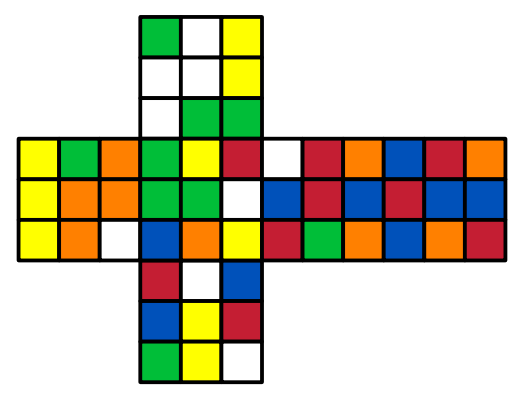
\includegraphics[width=8cm]{img/cubes/cub-barrejat.png}
    \caption{Cub barrejat per exemple de Memorització}
    \label{fig:exemple-memo}
    \end{figure}




\newpage
\section{Mètode Intermig (M2/Orozco)}

El mètode intermig per resoldre el cub a cegues consta del mètode M2 per les arestes i l'Orozco per les cantonades.
El mètode M2, que com ja ho diu el seu nom es basa en el moviment M2, que és el moviment de la capa del mig del cub 2 vegades, a més a més, el buffer és UK (Aresta )

\begin{figure}[h]
    \centering\RubikCubeSolvedWY
    \RubikRotation{Y,M2}
    \ShowCube{7cm}{0.7}{\DrawRubikCubeLU}
    \caption{Exemple de Moviment M2}
\end{figure}
    
Aquest mètode intercanvia les peces d'una manera peculiar, ja que ha de fer dues vegades M2 per tornar a l'estat original i canviar dues peces. Per exemple, fas primer la seqüència Y que col·loca la peça al lloc d'intercanvi, després fas la seqüència X que en aquesta cas és M2 i després fas Y' per retornar la peça intercanviada. Un cop fet això s'han canviat dues peces però el cub no queda igual que abans perquè hem de tornar a fer un intercanvi, aquest segon intercanvi ha de ser amb una seqüència Z X Z' perquè hem d'intercanviar una peça que no sigui la mateixa.\\\\Exemple d'intercanvi d'arestes L i V:

\begin{figure}[htbp]
    \centering
    \begin{subfigure}
        \centering\RubikCubeSolvedWY
        \RubikRotation{Y,Up,Lp,U}
        \ShowCube{7cm}{0.5}{\DrawRubikCubeRU}
    \end{subfigure}
    \begin{subfigure}
        \centering\RubikCubeSolvedWY
        \RubikRotation{Y,Up,Lp,U,M2}
        \ShowCube{7cm}{0.5}{\DrawRubikCubeRU}
    \end{subfigure}
    \caption{Secuencia Y (Esquerra) i Y X (Dreta)}
\end{figure}

\begin{figure}[htbp]
    \centering
    \begin{subfigure}
        \centering\RubikCubeSolvedWY
        \RubikRotation{Y,Up,Lp,U,M2,Up,L,U}
        \ShowCube{7cm}{0.5}{\DrawRubikCubeRU}
    \end{subfigure}
    \begin{subfigure}
        \centering\RubikCubeSolvedWY
        \RubikRotation{Y,Up,Lp,U,M2,Up,L,U,U,R2,Up}
        \ShowCube{7cm}{0.5}{\DrawRubikCubeRU}
    \end{subfigure}
    \caption{Secuencia Y X Y' (Esquerra) i Y X Y'Z (Dreta)}
\end{figure}

\begin{figure}[h!]
    \centering
    \begin{subfigure}
        \centering\RubikCubeSolvedWY
        \RubikRotation{Y,Up,Lp,U,M2,Up,L,U,U,R2,Up,M2}
        \ShowCube{7cm}{0.5}{\DrawRubikCubeRU}
    \end{subfigure}
    \begin{subfigure}
        \centering\RubikCubeSolvedWY
        \RubikRotation{Y,Up,Lp,U,M2,Up,L,U,U,R2,Up,M2,U,R2,Up}
        \ShowCube{7cm}{0.5}{\DrawRubikCubeRU}
    \end{subfigure}
    \caption{Secuencia Y X Y'Z'X (Esquerra) i Y X Y'Z X Z' (Dreta)}
\end{figure}

Llavors així és com es canviarien dues arestes amb el mètode M2, en aquest cas L i V. El mètode té els casos de la taula \ref{fig:taula-m2}.

\begin{table}[h]
    \begin{minipage}{.5\linewidth}
        \centering
        \begin{tabular}{|c|c|}
            \hline
            A & M2 \\
            \hline
            B & R' U R U' M2 U R' U' R \\
            \hline
            C & U2 M' U2 M' \\
            \hline
            D & L U' L' U M2 U' L U L'  \\
            \hline
            E & B L' B' M2 B L B'  \\
            \hline
            F & B L2 B' M2 B L2 B' \\
            \hline
            G & B L B' M2 B L' B' \\
            \hline
            H & L B L' B' M2 B L B' L' \\
            \hline
            I & D M' U R2 U' M U R2 U' D' M2 \\
            \hline
            J & U R U' M2 U R' U' \\
            \hline
            K & Posició d'intercanvi \\
            \hline
            L & U' L' U M2 U' L U \\
            \hline 
        \end{tabular}
    \end{minipage}
    \begin{minipage}{.5\linewidth}
        \centering
        \begin{tabular}{|c|c|}
            \hline
             M & B' R B M2 B' R' B \\
             \hline
             N & R' B' R B M2 B' R' B R  \\
             \hline
             O & B' R' B M2 B' R B \\
             \hline
             P & B' R2 B M2 B' R2 B \\
             \hline
             Q & U B' R U' B (M2) B' U R' B U' \\
             \hline
             R & U' L U M2 U' L' U \\
             \hline
             S & M2' D U R2 U' M' U R2 U' M D' \\
             \hline
             T & U R' U' M2 U R U'  \\
             \hline
             U & Posició d'intercanvi \\
             \hline
             V & U R2 U' M2 U R2 U' \\
             \hline
             W & M U2 M U2  \\
             \hline
             X & U' L2 U M2 U' L2 U \\
             \hline 
        \end{tabular}
    \end{minipage} 
    \caption{Casos del Mètode M2}
    \label{fig:taula-m2}
\end{table}


\subsection{Mètode d'execució per les Cantonades}

El mètode orozco, utlitza un sistema similar al M2, ja que fa les seqüències Y X Y'X' i Z A Z' A' però en aquest cas la seqüència Z és diferent perquè es troba al segon lloc. De manera simple, si a la memorització tens la lletra en segon lloc has de fer l'algoritme alternatiu.
Els casos d'orozco són els de la taula \ref{fig:taula-orozco}

\begin{table}[!h]
    \begin{minipage}{.5\linewidth}
        \centering
        \begin{tabular}{|c|c|} 
            \hline
            \textbf{AB} & Basic A Perm \\
            \hline
            \textbf{DB} & U' (A Perm) U \\
            \hline
            \textbf{EB} & [R: [R D R', U]] \\
            \hline
            \textbf{FB} & [R': [U', R' D' R]] \\
            \hline
            \textbf{GB} & [U, R' D R] \\
            \hline
            \textbf{HB} & [R D' R', U'] \\
            \hline
            \textbf{IB} & [R: [R D R', U2]] \\
            \hline
            \textbf{KB} & [D': [U, R' D R]] \\
            \hline
            \textbf{LB} & [D: [U, R' D' R]] \\
            \hline
            \textbf{OB} & [R D R', U'] \\
            \hline
            \textbf{PB} & [U, R' D' R] \\
            \hline
            \textbf{RB} & [R': [U2, R' D' R]] \\
            \hline
            \textbf{SB} & [U, R' D2 R] \\
            \hline
            \textbf{TB} & [D: [R D' R', U']] \\
            \hline
            \textbf{UB} & [x': [R U R', D2]] \\
            \hline
            \textbf{VB} & [D' x': [R U R', D2]] \\
            \hline
            \textbf{WB} & [D x: [D2, R' U' R]] \\
            \hline
            \textbf{XB} & [x: [D2, R' U' R]] \\
            \hline 
        \end{tabular}
    \end{minipage}
    \begin{minipage}{.5\linewidth}
        \centering
        \begin{tabular}{|c|c|}
            \hline
            \textbf{BA} & Reverse A Perm \\
            \hline
            \textbf{BD} & U' (Reverse A Perm) U \\
            \hline
            \textbf{BE} & [R: [U, R D R']] \\
            \hline
            \textbf{BF} & [R': [R' D' R, U']] \\
            \hline
            \textbf{BG} & [R' D R, U] \\
            \hline
            \textbf{BH} & [U', R D' R'] \\
            \hline
            \textbf{BI} & [R: [U2, R D R']] \\
            \hline
            \textbf{BK} & [D': [R' D R, U]] \\
            \hline
            \textbf{BL} & [D: [R' D' R, U]] \\
            \hline
            \textbf{BO} & [U', R D R'] \\
            \hline
            \textbf{BP} & [R' D' R, U] \\
            \hline
            \textbf{BR} & [R': [R' D' R, U2]] \\
            \hline
            \textbf{BS} & [R' D2 R, U] \\
            \hline
            \textbf{BT} & [D: [U', R D' R']] \\
            \hline
            \textbf{BU} & [x': [D2, R U R']] \\
            \hline
            \textbf{BV} & [D' x': [D2, R U R']] \\
            \hline
            \textbf{BW} & [D x: [R' U' R, D2]] \\
            \hline
            \textbf{BX} & [x: [R' U' R, D2]] \\
            \hline 
        \end{tabular}
    \end{minipage} 
    \caption{Algorimtes orozco}
    \label{fig:taula-orozco}
\end{table}

A la columna de l'esquerra hi ha els corresponents a la primera lletra del parell i a la dreta els corresponents a la segona lletra del parell. \textit{A perm} és un cas del cub de rubik normal que es fa (R' U' R' D' R U' R' D R U R' D' R U R' D R2).
Cal tambe tenir en compte que els algoritmes estan una notació diferents perquè es vegi de millor forma al ser tants algoritmes. Funciona de la següent manera [A,B] = A,B,A',B'.

\begin{table}[h]
    \begin{minipage}{.5\linewidth}
        \centering
        \begin{tabular}{|c|c|}
            \hline
            \textbf{NB} & [U, R' D R D' R' D' R] \\
            \hline
            \textbf{QB} & [R' D R D' R' D' R, U] \\
            \hline
        \end{tabular}
    \end{minipage}
    \begin{minipage}{.5\linewidth}
        \centering
        \begin{tabular}{|c|c|}
            \hline
            \textbf{BN} & [R' D R D' R' D' R, U] \\
            \hline
            \textbf{BQ} & [U, R' D R D' R' D' R] \\
            \hline 
        \end{tabular}
    \end{minipage} 
    \caption{Excepcions del mètode}
\end{table}



Aquests algoritmes estan escrits en una notació\footnote{Manera d'escriure els algoritmes} diferenti [Y,X]. El fet que estigui entre claudators indica que s'ha de fer en l'ordre Y X Y' X'. És una mica més díficil de visualitzar però més fàcil a l'hora d'aplicar aquest mètode.
Exepmle d'intercanvi de dues cantonades P i H

\begin{figure}[h!]
    \centering
    \begin{subfigure}
        \centering\RubikCubeSolvedWY
        \RubikRotation{Y,U}
        \ShowCube{7cm}{0.5}{\DrawRubikCubeLU}
    \end{subfigure}
    \begin{subfigure}
        \centering\RubikCubeSolvedWY
        \RubikRotation{Y,U,Rp,Dp,R}
        \ShowCube{7cm}{0.5}{\DrawRubikCubeLU}
    \end{subfigure}
    \caption{Secuencia Y (Esquerra) i Y X (Dreta)}
\end{figure}

\begin{figure}[h!]
    \centering
    \begin{subfigure}
        \centering\RubikCubeSolvedWY
        \RubikRotation{Y,U,Rp,Dp,R,Up}
        \ShowCube{7cm}{0.5}{\DrawRubikCubeLU}
    \end{subfigure}
    \begin{subfigure}
        \centering\RubikCubeSolvedWY
        \RubikRotation{Y,U,Rp,Dp,R,Up,Rp,D,R}
        \ShowCube{7cm}{0.5}{\DrawRubikCubeLU}
    \end{subfigure}
    \caption{Secuencia Y X Y' (Esquerra) i Y X Y' X'(Dreta)}
\end{figure}

\begin{figure}[h!]
    \centering
    \begin{subfigure}
        \centering\RubikCubeSolvedWY
        \RubikRotation{Y,U,Rp,Dp,R,Up,Rp,D,R,Up}
        \ShowCube{7cm}{0.5}{\DrawRubikCubeLU}
    \end{subfigure}
    \begin{subfigure}
        \centering\RubikCubeSolvedWY
        \RubikRotation{Y,U,Rp,Dp,R,Up,Rp,D,R,Up,R,Dp,Rp}
        \ShowCube{7cm}{0.5}{\DrawRubikCubeLU}
    \end{subfigure}
    \caption{Secuencia Y X Y' X' Z (Esquerra) i Y X Y' X' Z A(Dreta)}
\end{figure}

\begin{figure}[h!]
    \centering
    \begin{subfigure}
        \centering\RubikCubeSolvedWY
        \RubikRotation{Y,U,Rp,Dp,R,Up,Rp,D,R,Up,R,Dp,Rp,U}
        \ShowCube{7cm}{0.5}{\DrawRubikCubeLU}
    \end{subfigure}
    \begin{subfigure}
        \centering\RubikCubeSolvedWY
        \RubikRotation{Y,U,Rp,Dp,R,Up,Rp,D,R,Up,R,Dp,Rp,U,R,D,Rp}
        \ShowCube{7cm}{0.5}{\DrawRubikCubeLU}
    \end{subfigure}
    \caption{Secuencia Y X Y' X' Z A Z' (Esquerra) i Y X Y' X' Z A Z' A'(Dreta)}
\end{figure}

Com a orientació [Y,X] i [Z,A] són a la taula d'algoritmes PB i BH.

\newpage
\large{Fins aquí el tutorial de 3BLD, espero que hagi sigut de fàcil comprensió i que t'hagi ajudat a resoldre el cub a cegues.}

\newpage
\begin{table}[h]
    \centering
    \begin{tabular}{|l|l|l|l|}
    \hline
    AA & AA                 & BL & BL                      \\ \hline
    AB & ABS                & BM & BM (spam)               \\ \hline
    AC & Aire Acondicionat  & BN & BiNari                  \\ \hline
    AD & AD (Anunci)        & BO & BOB                     \\ \hline
    AE & Aero               & BP & BP (gasolinera)         \\ \hline
    AF & AFRO               & BQ & BQ (marca de mòbils)    \\ \hline
    AG & AG (PLATA)         & BR & BRR (so)                \\ \hline
    AH & AHORA              & BS & BS (abreviació de text) \\ \hline
    AI & AI (Onomatopeia)   & BT & BlueTooth               \\ \hline
    AJ & AJO                & BU & BU (so)                 \\ \hline
    AK & AK-47              & BV & BBVA                    \\ \hline
    AL & ALUMINI            & BW & BBW (brake by wire)     \\ \hline
    AM & AM                 & BX & BoX                     \\ \hline
    AN & AN                 & CA & Catalunya               \\ \hline
    AO & AVERAGE OF         & CB & CB (defensa central)    \\ \hline
    AP & APP                & CC & CC (correu)             \\ \hline
    AQ & AQuaman            & CD & CD                      \\ \hline
    AR & AR SPEEDCUBER      & CE & CEo                     \\ \hline
    AS & AS                 & CF & CoFre                   \\ \hline
    AT & AlphaTauri         & CG & Centre de Gravetat      \\ \hline
    AU & AU (Onomatopeia)   & CH & CHili                   \\ \hline
    AV & AVE                & CI & CI (compl indirecte)    \\ \hline
    AW & AWard              & CJ & CJ                      \\ \hline
    AX & AXE                & CK & CooK                    \\ \hline
    BA & BALA               & CL & ClocK                   \\ \hline
    BB & BEBÉ               & CM & Càmera                  \\ \hline
    BC & BC (Before Christ) & CN & CN (compl nom)          \\ \hline
    BD & BuD                & CO & CO (companyia)          \\ \hline
    BE & Bed                & CP & Codi Postal             \\ \hline
    BF & BFF                & CQ & CaQui                   \\ \hline
    BG & BackGround         & CR & CR (continental record) \\ \hline
    BH & BH (BICICLETES)    & CS & CS (computer science)   \\ \hline
    BI & BI                 & CT & CTT                     \\ \hline
    BJ & BeiJing            & CU & CUb                     \\ \hline
    BK & BreaK              & CV & CV (curric.vitae)       \\ \hline
    \end{tabular}
    \caption{Taula de Parells de Lletres AA \rightarrow CV}
    \label{tla:lletres-1}
    \end{table}

\begin{table}[h]
    \centering
    \begin{tabular}{llll}
    \hline
    CW & CoW               & EJ & EJect                 \\ \hline 
    CX & CX (Citroen)      & EK & EKA (mètode)          \\ \hline
    DA & DA (sí en Rus)    & EL & EL                    \\ \hline
    DB & DataBase          & EM & Eminem                \\ \hline
    DC & DC (Distr of C)   & EN & EN                    \\ \hline
    DD & DoDo              & EO & EO (edge orientation) \\ \hline
    DE & DE                & EP & EP                    \\ \hline
    DF & Districte Federal & EQ & EquiP                 \\ \hline
    DG & DoG               & ER & ER (European record)  \\ \hline
    DH & DHl               & ES & Espanya               \\ \hline
    DI & DIA               & ET & ET                    \\ \hline
    DJ & DJ                & EU & Estats Units          \\ \hline
    DK & Donkey Kong       & EV & EVO                   \\ \hline
    DL & DòLar             & EW & EW (so)               \\ \hline
    DM & DuMb              & EX & EX                    \\ \hline
    DN & DaN               & FA & Fa (nota musical)     \\ \hline
    DO & DO (nota musical) & FB & FaceBook              \\ \hline
    DP & DP (empresa)      & FC & FC (futbol club)      \\ \hline
    DQ & DsQ               & FD & Feed                  \\ \hline
    DR & Domino Reduction  & FE & FE                    \\ \hline
    DS & DS (Nintendo)     & FF & ForceFeedback         \\ \hline
    DT & DoT               & FG & FueGo                 \\ \hline
    DU & DUo               & FH & FarenHeit             \\ \hline
    DV & DaVid             & FI & FInlandia             \\ \hline
    DW & DeU               & FJ & FiJi                  \\ \hline
    DX & DuX               & FK & FaKe                  \\ \hline
    EA & EA (empresa)      & FL & FLuid                 \\ \hline
    EB & EB (Buggati)      & FM & FM (radio)            \\ \hline
    EC & ECo               & FN & FortNite              \\ \hline
    ED & Educació          & FO & FOca                  \\ \hline
    EE & EE (so)           & FP & FP                    \\ \hline
    EF & EFecte            & FQ & FaQ                   \\ \hline
    EG & EG (mètode)       & FR & FRança                \\ \hline
    EH & EH (so)           & FS & For Speed             \\ \hline
    EI & Einstein          & FT & Foto                  \\ \hline  
    \end{tabular}
    \caption{Taula de Parells de Lletres CW \rightarrow FT}
    \label{tla:lletres-2}
    \end{table}


\begin{table}[h]
    \centering
    \begin{tabular}{l|l|l|l}
    FU & FUm            & HH & Hula Hop             \\\hline
    FV & FiVerr         & HI & HIppie               \\\hline
    FW & ForWard        & HJ & HiJo                 \\\hline
    FX & FaX            & HK & Honk Kong            \\\hline
    GA & GA (perm)      & HL & HaLo                 \\\hline
    GB & GB (perm)      & HM & HuM                  \\\hline
    GC & GC (perm)      & HN & HaN                  \\\hline
    GD & GoD            & HO & Ho Ho                \\\hline
    GE & GEl            & HP & HP (marca)           \\\hline
    GF & GiF            & HQ & High Quality         \\\hline
    GG & GG             & HR & Heart Rate           \\\hline
    GH & GraHam         & HS & High School          \\\hline
    GI & GIrona         & HT & HoT                  \\\hline
    GJ & Good Job       & HU & HUngary              \\\hline
    GK & GoKu           & HV & HaVe                 \\\hline
    GL & GL             & HW & HomeWork             \\\hline
    GM & Grand Master   & HX & HeXA                 \\\hline
    GN & GaN            & IA & IA (chatgpt)         \\\hline
    GO & GO             & IB & IBai                 \\\hline
    GP & Gran Premi     & IC & ICono                \\\hline
    GQ & GRAN QUESO     & ID & ID                   \\\hline
    GR & Grup           & IE & Internet Explorer    \\\hline
    GS & GaS            & IF & IF (condicional)     \\\hline
    GT & Gran Turismo   & IG & InstaGram            \\\hline
    GU & GUI            & IH & IdaHo                \\\hline
    GV & GraVa          & II & HawaII               \\\hline
    GW & Glow           & IJ & Injust               \\\hline
    GX & GX (opera GX)  & IK & IKea                 \\\hline
    HA & HAHA           & IL & ILL                  \\\hline
    HB & HB (llapis)    & IM & International Master \\\hline
    HC & HeliCòpter     & IN & IN                   \\\hline
    HD & HD (resolució) & IO & IÓ (química)         \\\hline
    HE & HE (pronom)    & IP & IP                   \\\hline
    HF & HiFi           & IQ & IQ                   \\\hline
    HG & HuG            & IR & InfraRoig            \\\hline
    \end{tabular}
    \caption{Taula de Parells de Lletres FU \rightarrow IR}
    \label{tla:lletres-3}
    \end{table}

\begin{table}[h]
    \centering
    \begin{tabular}{|l|l|l|l|}
    \hline
    IS & ISs                    & KF & KFc            \\ \hline
    IT & ITalia                 & KG & KiloGram       \\ \hline
    IU & InUiT                  & KH & Kevin Hays     \\ \hline
    IV & \multicolumn{1}{r|}{4} & KI & Kit            \\ \hline
    IW & IntervieW              & KJ & KiloJoule      \\ \hline
    IX & \multicolumn{1}{r|}{9} & KK & KK             \\ \hline
    JA & JA (perm)              & KL & Kuala Lumpur   \\ \hline
    JB & JB (perm)              & KM & KilòMetre      \\ \hline
    JC & JaCuzzi                & KN & KeNtucky       \\ \hline
    JD & JD (sports)            & KO & KOi            \\ \hline
    JE & JErry                  & KP & KaPPa          \\ \hline
    JF & JeFF                   & KQ & KaQui          \\ \hline
    JG & Jaguar                 & KR & Korea          \\ \hline
    JH & JoHn                   & KS & KiSs  (grup)   \\ \hline
    JI & JedI                   & KT & KaTana         \\ \hline
    JJ & JJ                     & KU & KUwait         \\ \hline
    JK & JoKer                  & KV & KeVin          \\ \hline
    JL & JuLiol                 & KW & KiWi           \\ \hline
    JM & JaM                    & KX & KlineX         \\ \hline
    JN & JaN                    & LA & Los Ángeles    \\ \hline
    JO & JOe                    & LB & Left Back      \\ \hline
    JP & JP                     & LC & LuCk           \\ \hline
    JQ & JQuery                 & LD & Lateral Dret   \\ \hline
    JR & JunioR                 & LE & LE             \\ \hline
    JS & JeSús                  & LF & LeaF           \\ \hline
    JT & JeT                    & LG & LG (marca)     \\ \hline
    JU & JUny                   & LH & Lewis Hamilton \\ \hline
    JV & Java                   & LI & LI             \\ \hline
    JW & JeW                    & LJ & LumberJack     \\ \hline
    JX & JinX                   & LK & LiKe           \\ \hline
    KA & KaYak                  & LL & LLimona        \\ \hline
    KB & KirBy                  & LM & Lichess Master \\ \hline
    KC & KC                     & LN & Lando Norris   \\ \hline
    KD & KD (nba)               & LO & Lo             \\ \hline
    KE & KEy                    & LP & LuPa           \\ \hline
    \end{tabular}
    \caption{Taula de Parells de Lletres IS \rightarrow LP}
    \label{tla:lletres-4}
    \end{table}

\begin{table}[h]
    \centering
    \begin{tabular}{|l|l|l|l|}
    \hline
    LQ & LoQuendo       & ND & NaDa                 \\ \hline
    LR & Left-Right     & NE & NEo                  \\ \hline
    LS & LàSer          & NF & NeFast               \\ \hline
    LT & LiT            & NG & Negre                \\ \hline
    LU & LU             & NH & Nothing              \\ \hline
    LV & LaVa           & NI & NInja                \\ \hline
    LW & LoW            & NJ & NíJar                \\ \hline
    LX & LateX          & NK & NoKia                \\ \hline
    MA & MAma           & NL & NetherLands          \\ \hline
    MB & MBappé         & NM & NeMo                 \\ \hline
    MC & MigCampista    & NN & NN                   \\ \hline
    MD & MD (missatge)  & NO & NO                   \\ \hline
    ME & MEme           & NP & NPc                  \\ \hline
    MF & MaFia          & NQ & NesQuick             \\ \hline
    MG & MaGnesi        & NR & NR (National Record) \\ \hline
    MH & MoHa           & NS & No-Sé                \\ \hline
    MI & MI             & NT & NATA                 \\ \hline
    MJ & Michael Jordan & NU & NUt                  \\ \hline
    MK & MK             & NV & November             \\ \hline
    ML & MaiL           & NW & NeWs                 \\ \hline
    MM & MaMut          & NX & NeXt                 \\ \hline
    MN & MaNia          & OA & OAk (tronc)          \\ \hline
    MO & MO             & OB & OBama                \\ \hline
    MP & Max ParK       & OC & Oceania              \\ \hline
    MQ & MaQueta        & OD & ODD                  \\ \hline
    MR & MisteR         & OE & OEm                  \\ \hline
    MS & MeSSi          & OF & OFICINA              \\ \hline
    MT & MiT            & OG & OG                   \\ \hline
    MU & MUU            & OH & One Handed           \\ \hline
    MV & MagleV         & OI & OI                   \\ \hline
    MW & MicroWave      & OJ & OJO                  \\ \hline
    MX & MèXic          & OK & OK                   \\ \hline
    NA & Na (perm)      & OL & Olímpic              \\ \hline
    NB & NBa            & OM & OMAR                 \\ \hline
    NC & NiCe           & ON & ON                   \\ \hline
    \caption{Taula de Parells de Lletres LQ \rightarrow ON}
    \label{tla:lletres-5}
    \end{tabular}
    \end{table}    

\begin{table}[h]
    \centering
    \begin{tabular}{|l|l|l|l|}
    \hline
    OO & OO                    & QB & QuarterBack      \\ \hline
    OP & Old Pochmann          & QC & QualComm         \\ \hline
    OQ & ORQUESTA              & QD & QuaD             \\ \hline
    OR & Olimpic Record        & QE & QuE              \\ \hline
    OS & OS (sistema operatiu) & QF & QuiròFan         \\ \hline
    OT & OT                    & QG & QuirúrGic        \\ \hline
    OU & OU                    & QH & sQuasH           \\ \hline
    OV & OVni                  & QI & QuI              \\ \hline
    OW & OW                    & QJ & QuiJote          \\ \hline
    OX & OXígen                & QK & QuaKer           \\ \hline
    PA & PA                    & QL & Quality          \\ \hline
    PB & PB (Personal Best)    & QM & QuantuM          \\ \hline
    PC & PC                    & QN & QuaN             \\ \hline
    PD & Post Data             & QO & QuOte            \\ \hline
    PE & PE                    & QP & eQuiP            \\ \hline
    PF & PFI                   & QQ & QQ               \\ \hline
    PG & PGa (Golf)            & QR & QR (Codi)        \\ \hline
    PH & PH (àcid)             & QS & QuickSilver      \\ \hline
    PI & PI (π)                & QT & QuarenTena       \\ \hline
    PJ & PiJama                & QU & QU               \\ \hline
    PK & PeKKA                 & QV & eQuiVocar        \\ \hline
    PL & PoLand                & QW & QWerty           \\ \hline
    PM & PM (hora)             & RA & RA (perm)        \\ \hline
    PN & PeN                   & RB & RedBull          \\ \hline
    PO & POl                   & RC & Radio Control    \\ \hline
    PP & PP                    & RD & RD (País)        \\ \hline
    PQ & Pecús                 & RE & REd              \\ \hline
    PR & PR (Personal Record)  & RF & RaFa             \\ \hline
    PS & PlayStation           & RG & NRG              \\ \hline
    PT & PorTugal              & RH & RuiHang          \\ \hline
    PU & PUma                  & RI & RIu              \\ \hline
    PV & PVc                   & RJ & RJ-44 (ethernet) \\ \hline
    PW & PoWer                 & RK & RocK             \\ \hline
    PX & PiXel                 & RL & Rocket League    \\ \hline
    QA & QAtar                 & RM & RaM (cotxe)      \\ \hline
    \caption{Taula de Parells de Lletres OO \rightarrow RM}
    \label{tla:lletres-6}
    \end{tabular}
    \end{table}

\begin{table}[h]
    \centering
    \begin{tabular}{|l|l|l|l|}
    \hline
    RN & Right now              & TA & TATA                  \\ \hline
    RO & ROda                   & TB & TaBleT                \\ \hline
    RP & RaP                    & TC & TC (Traction Control) \\ \hline
    RQ & RaQueta                & TD & TeD                   \\ \hline
    RR & RaRo                   & TE & TÉ                    \\ \hline
    RS & RS (Rally Sport)       & TF & TelèFon               \\ \hline
    RT & RT (retweet)           & TG & TiGer                 \\ \hline
    RU & Rusia                  & TH & THomb                 \\ \hline
    RV & RoVer                  & TI & TI                    \\ \hline
    RW & RoW                    & TJ & TaJo                  \\ \hline
    RX & ReX                    & TK & TicKet                \\ \hline
    SA & Sud-Àfrica             & TL & TeLa                  \\ \hline
    SB & SportBack              & TM & TeaM                  \\ \hline
    SC & SoniC                  & TN & TNt                   \\ \hline
    SD & SD (resolució)         & TO & TOnelada              \\ \hline
    SE & SEa                    & TP & TP                    \\ \hline
    SF & SoFà                   & TQ & TorQue                \\ \hline
    SG & SaGa                   & TR & TRx                   \\ \hline
    SH & SHHHH                  & TS & TypeScript            \\ \hline
    SI & SI                     & TT & TT                    \\ \hline
    SJ & SoJa                   & TU & TU                    \\ \hline
    SK & SKi                    & TV & TV                    \\ \hline
    SL & SL (Societat Limitada) & TW & TWitch                \\ \hline
    SM & SM (Editorial)         & TX & TaXi                  \\ \hline
    SN & SN (Sense Número)      & UA & UA (Uni Autònoma BCN) \\ \hline
    SO & SO                     & UB & UB (Uni BCN)          \\ \hline
    SP & SPort                  & UC & UCrania               \\ \hline
    SQ & SQuare                 & UD & UDemy (cursos)        \\ \hline
    SR & SR (State Record)      & UE & Unió Europea          \\ \hline
    SS & SS                     & UF & UFo                   \\ \hline
    ST & STreet                 & UG & UdG (Uni Girona)      \\ \hline
    SU & SUpra                  & UH & UpHill                \\ \hline
    SV & SuV                    & UI & UI (user interface)   \\ \hline
    SW & Star Wars              & UJ & Utah Jazz             \\ \hline
    SX & SaXo (cotxe)           & UK & UK (país)             \\ \hline
    \caption{Taula de Parells de Lletres RN \rightarrow UK}
    \label{tla:lletres-7}
    \end{tabular}
    \end{table}

\begin{table}[h]
    \centering
    \begin{tabular}{|l|l|l|l|}
    \hline
    UL & ULtron               & VW & VolksWagen        \\ \hline
    UM & fUM                  & VX & VorteX            \\ \hline
    UN & UNo                  & WA & WAter             \\ \hline
    UO & UndercOver           & WB & WeB               \\ \hline
    UP & Up                   & WC & WC                \\ \hline
    UQ & UniQue               & WD & WD (discos)       \\ \hline
    UR & URuguai              & WE & WWE               \\ \hline
    US & US (país)            & WF & WiFi              \\ \hline
    UT & U-Turn               & WG & WinG              \\ \hline
    UU & UU                   & WH & WasH              \\ \hline
    UV & UtrolaViolat         & WI & WII               \\ \hline
    UW & UW                   & WJ & WaterJet          \\ \hline
    UX & UNIX                 & WK & WiKipedia         \\ \hline
    VA & VA                   & WL & WiLL              \\ \hline
    VB & VerB                 & WM & WRM (cub)         \\ \hline
    VC & VaCa                 & WN & WiN               \\ \hline
    VD & ViDeo                & WO & WOOo              \\ \hline
    VE & VErstappen           & WP & WeaPon            \\ \hline
    VF & VeriFicar            & WQ & WuQue (cub)       \\ \hline
    VG & VaGo                 & WR & WR (World Record) \\ \hline
    VH & VHS                  & WS & WhatSapp          \\ \hline
    VI & VI                   & WT & What              \\ \hline
    VJ & VaJa                 & WU & WU                \\ \hline
    VK & ValK                 & WV & WolVerine         \\ \hline
    VL & VoLar                & WW & WWW               \\ \hline
    VM & ViM                  & WX & WAX               \\ \hline
    VN & VaNs                 & XA & EXamen            \\ \hline
    VO & VO (Versió Original) & XB & XBox              \\ \hline
    VP & ViP                  & XC & eXCel             \\ \hline
    VQ & VAnQuish             & XD & XD                \\ \hline
    VR & VR                   & XE & XEon (intel)      \\ \hline
    VS & VerSus               & XF & XilòFon           \\ \hline
    VT & VoT                  & XG & EXtra Gran        \\ \hline
    VU & VUVUzela             & XH & EXHalar           \\ \hline
    VV & VàlVula              & XI & XI                \\ \hline
    \end{tabular}
    \caption{Taula de Parells de Lletres UL \rightarrow XI}
    \label{tla:lletres-8}
    \end{table}  

\begin{table}[h]
    \centering
    \begin{tabular}{|l|l|l|l|}
    \hline
    XJ & EXiGir* (So) & XQ & Per Què     \\ \hline
    XK & XK           & XR & XR (iphone) \\ \hline
    XL & XL (talla)   & XS & XS (iphone) \\ \hline
    XM & X-Men        & XT & XTreme      \\ \hline
    XN & Xenó         & XU & XU          \\ \hline
    XO & ShO          & XV & XaVi        \\ \hline
    XP & XP (windows) & XW & XWing       \\ \hline
    XX   & XX              &  &          \\ \hline
    \end{tabular}
    \caption{Taula de Parells de Lletres XJ \rightarrow XX}
    \label{tla:lletres-9}
    \end{table}







\end{document}
